\documentclass{article}
\usepackage{graphicx}
\usepackage{url}
\usepackage[backend=biber]{biblatex}
\usepackage{fontspec}
\setmainfont{Latin Modern Roman}

\addbibresource{jhammond_final_report.bib}

\author{John Hammond}
\title{TE 401 Final Presentation FA19}

\begin{document}

%title followed by blank space before next pager
\maketitle
\tableofcontents
\newpage

%introduction and background on the project
\section{Motivation for the Augmented Listening Project}
Augmented listening and the work we are doing here will change the way we hear and perceive\
the world around us. The idea of augmented listening is to utilize microphone arrays of any size to alter the way we hear audio.\
Effects such as source separation, dynamic range compression, and selective attenuation are all examples of digital signal\
processing in the context of hearing. Devices like hearing aids are very common and help people by amplifying the sounds around\
them and performing basic dynamic range compression.  Hearing aids, however, are limited in their capabilities due to the small\
number of microphones available and the relatively small amount of processing power. They struggle in loud environments\
with multiple sources as well as reverberant environments.  Hearing aids are only one example of augmented listening\
technology, and applications go far beyond this.

We aim to create\
an open hardware platform with support for large numbers of microphones and complex signal processing algorithms.\
This hardware platform will function as a proof of concept for our own signal processing applications as well as those\
of other researchers across the world.  The basic platform is based upon a Cyclone\textsuperscript{\textregistered{}}\
V SoC system, with support for both\
hardware logic and software applications on the ARM cores. Our implementation supports I2S microphone data streams as\
inputs for processing.

%descripton of current hardware
\section{Current Hardware Platform}

\subsection{FPGA}
The FPGA is programmed to receive I2S data, store samples in DDR3 memory buffers, and to support real-time\
signal processing cores.  We will mostly describe the hardware as it relates to recording.

\subsubsection{I2S}
Our array prototypes have all consisted of MEMS microphones, which send their bit stream over the I2S bus.\
We chose these microphones because they are very cheap and easy to prototype with. Two microphones share a sample\
clock, right/left select clock, power, and a data line. The right and left channel alternate sending their 16\
bit samples. These samples are then pieced together at the I2S master into a coherent right and left data\
stream. These master cores are implemented in the FPGA fabric. Refer to figure\
\ref{i2s_timing} for an example of\
a typical I2S data transfer.

\begin{figure}[ht]
	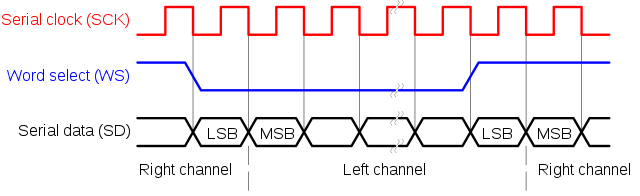
\includegraphics[scale=.5]{pictures/i2s_timing.png}
	\centering
	\caption{I2S timing diagram \cite{i2s}}
	\label{i2s_timing}
\end{figure}

\newpage

\subsubsection{Avalon\textsuperscript{\textregistered{}} Bus}
The Avalon\textsuperscript{\textregistered{}} bus is a wishbone style bus created by\
Altera\textsuperscript{\textregistered{}} to be used with their IP blocks.\
The basic connections on the Avalon\textsuperscript{\textregistered{}} bus are\
a single bit for read/write enable and 32 bits for read/write data. The bus supports\
more complex features such as burst transfers and wait requests by slave devices,\
but we have not needed to implement these. Future expansions of recording or\
processing algorithms may require faster data transfers, for which these additional\
features will become necessary.  See figure \ref{avalon} for a basic read and write\
transfer timing diagram.

\begin{figure}[ht]
	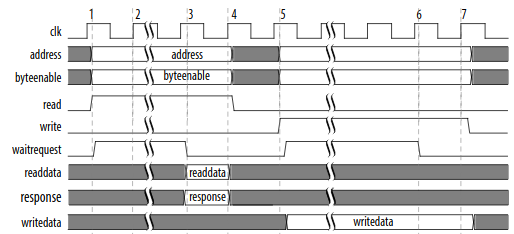
\includegraphics[scale=.5]{pictures/avalon.png}
	\centering

	\caption{Avalon\textsuperscript{\textregistered{}} read and write\
	timings \cite{avalon}}

	\label{avalon}
\end{figure}


\subsubsection{DMA Controller and Buffers}
Recording audio from a large number of microphones is a challenge and is one of the\
features of our\
open platform. There is 7.68 Mbit of space allocated in memory for the samples from\
each of the 10\
microphones. Each of the five I2S masters hold the latest valid 16-bit sample for each\
microphone on its output register. The DMA controller then iterates through these 10\
registers and writes their values to the proper memory address.  These data transfers\
are all done over the Avalon\textsuperscript{\textregistered{}} bus. \

Figure \ref{dma_sim} shows the activity on the\
Avalon\textsuperscript{\textregistered{}} bus while the DMA controller is running.\
The microphone sample data is asserted on the AM\_WRITEDATA line.  The address of each\
sample is asserted on the AM\_ADDR line.  The DMA controller cycles through these\
addresses while recording, as seen in the sequence of 0x1000024, 0x01753024,\
0x01EA6024, 0x025F9024, and 0x02D4C024. The write enable signal AM\_WRITE stays high\
for the duration of these transfers.

\begin{figure}[ht]
	\begin{center}
	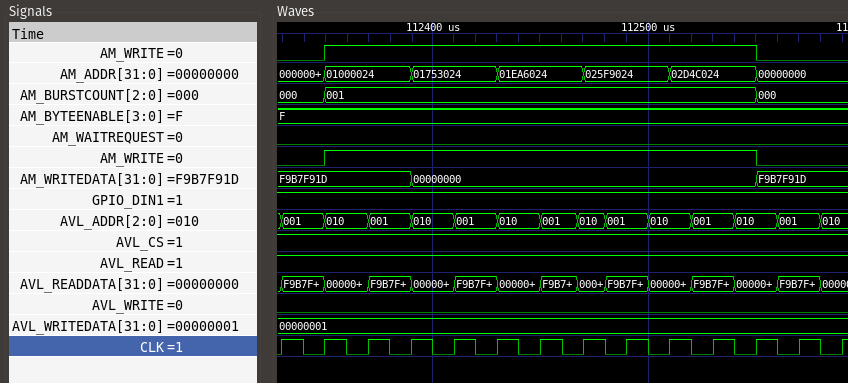
\includegraphics[scale=.38]{pictures/sim_close.png}
	\caption{Simulation of DMA access}
	\label{dma_sim}
	\end{center}
\end{figure}


% \subsubsection{Filtering}
% Real time signal processing can be performed in the FPGA fabric using hardware logic.\
% Altera\textsuperscript{\textregistered{}} provides FIR filters as part of their\
% university program.  

\subsection{HPS}

\subsubsection{Linux}
The hard processor system is based on two ARM Cortex-A9 cores.  On this processor we\ are running a lightweight GNU/Linux distribution to handle low level hardware control.\
File I/O, ftp, ssh, and ethernet controls are made very easy using the HPS as opposed\
to pure hardware logic. Altera\textsuperscript{\textregistered{}}'s provided OS image\
can be put on a microSD card and booted at power on.

\subsubsection{Recording and Processing}
On top of our Linux system we have a small C++ program to read samples from the DDR3\
buffer and store it or process it.  This is the second part of the recording process\
after the DDR3 buffers have been completely filled out by the DMA controller.\
This piece of code actually works similarly to the DMA in hardware just in\
reverse. 

Altera\textsuperscript{\textregistered{}} provides libraries with their HPS\
development environment to make the HPS interface nicer with the FPGA fabric.\
Specifically, the current recording program uses the ``mmap'' function to map the\
FPGA memory mapped addresses to addresses in the GNU/Linux userspace. These\
addresses are dereferenced in the C++ program to access the FPGA's hardware\
registers. This is more complex than using a soft core such as a RISC-V core\
or a ZipCPU because the hard processor cannot be reconfigured for each\
new hardware configuration. Figure \ref{mmap} shows an example embeded\
GNU/Linux memory map.

\begin{figure}[ht]
	\begin{center}
	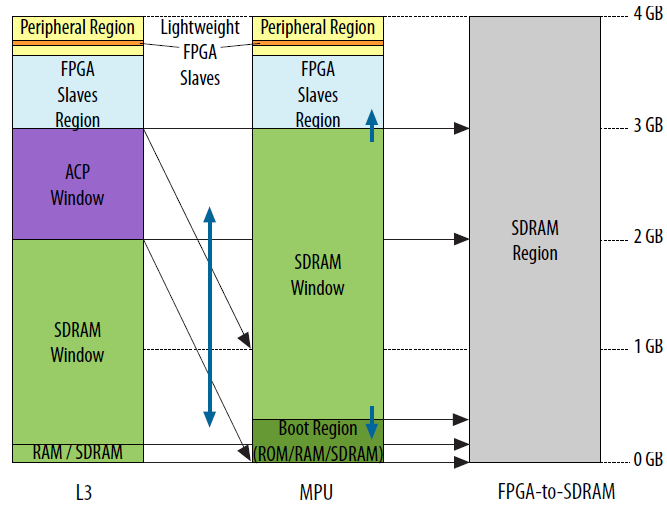
\includegraphics[scale=.38]{pictures/mmap.png}
	\caption{Embeded Linux memory map \cite{mmap}}
	\label{mmap}
	\end{center}
\end{figure}

The other major functions we utilize in\
recording are the ``alt\_read\_word'' and ``alt\_write\_words'' programs distributed by\
Altera\textsuperscript{\textregistered{}}. These functions have the sole purpose of\
writing and reading data over the Avalon bus. The write function takes the base\
address to write to and the data to write and will write that value on the\
Avalon bus. The read function works similarly, taking an address and returning the\
value read off the bus. 

These functions combined form the basic building blocks for the recording algorithm.\
In our recording program, we start by writing the start bit for the DMA state machine.\
The software recording loop then waits for the DMA controller to signify that the DDR3\
buffers have been fully filled out, after which it will begin fetching samples from\
the buffers and storing them to the microSD card. Figure \ref{dma_sim} shows these\
control signals labeled as AVL\_*.

Software digital signal processing on the HPS is another feature of our platform\
that will be useful for prototyping algorithms. The HPS does not have the same\
performance as dedicated hardware signal processing, but it is useful for prorotyping\
quick algorithms. This is especially useful because signal processing on personal\
computers is complicated by input drivers and operating system quirks.

\section{Going Forward}
The current hardware platform is functioning with a 10 microphone array and basic\
FIR filters implemented in hardware, but we still have improvements we would like\
to make before handing off the platform to other researchers.

\subsection{SignalTap\textsuperscript{\textregistered{}} and its Flaws}
The development of our current system has been done exclusively on the actual\
development board. SignalTap\textsuperscript{\textregistered{}} is the main tool\
used for debugging on the board. SignalTap\textsuperscript{\textregistered{}} works\
by instantiating a logic analyzer on the FPGA and sending the captures back to\
the computer over USB. Figure \ref{signaltap} shows a capture of recording on\
our physical board, the same signals seen in figure \ref{dma_sim}. This is a\
useful tool for doing final verification on the board, but it is cumbersome\
to use for rapid prototyping and developing new algorithms.\
SignalTap\textsuperscript{\textregistered{}} has two main drawbacks. First,\
SignalTap\textsuperscript{\textregistered{}} requires the design to be fully\
recompiled every time we want to look at new signals.  This is especially\
troublesome when compile times exceed 10 minutes, which they already do on\
our relatively simple platform. The other issue with\
SignalTap\textsuperscript{\textregistered{}} is the limit on capture time\
and signal widths. SignalTap\textsuperscript{\textregistered{}} works by\
capturing signals and storing the values on a block ram. Block ram is\
very fast, but it is extremely limited in size. The FPGA we are using\
has only 4.45 Mbits of block ram. This is quickly filled when we need to\
capture multiple 32 bit signals for any reasonable sample length.\
The solution to these problems is to do development in a software simulation\ 
environment.

\begin{figure}[ht]
	\begin{center}
	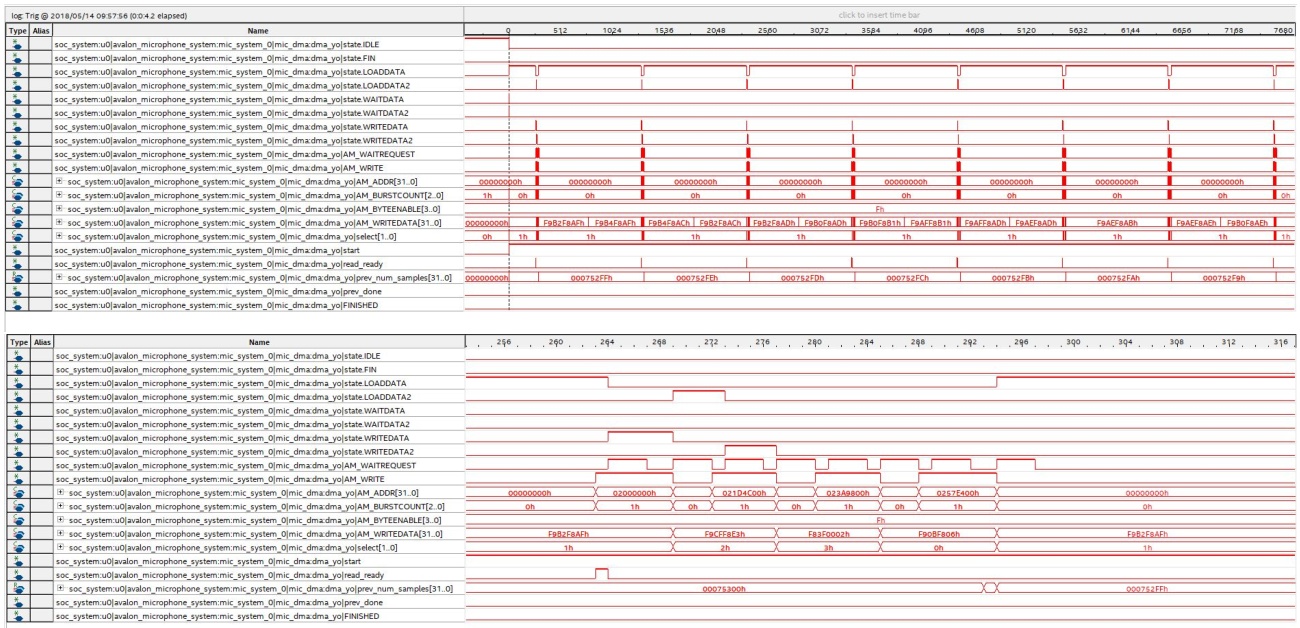
\includegraphics[scale=.28]{pictures/signaltap.png}
	\caption{SignalTap\textsuperscript{\textregistered} capture of DMA access from Juan\
	Martinez}
	\label{signaltap}
	\end{center}
\end{figure}

\subsection{Software Simulation and Verilator}
Software simulation allows us to quickly develop new algorithms and test them\
immediately in a performant simulation environment. The program we have chosen\
for our HDL simulation is Verilator. Verilator is an open source simulator\
that works using a cycle based model of the hardware logic. Verilator compiles\
a SystemVerilog design down to a C++ class, known as a ``verilated'' design,\
that can then be stimulated by auxiliary\
C++ code. Inputs and outputs of the design are exposed as public variables\
in the object. These can be stimulated by flipping bits individually and clocking\
the design in a similar way to ModelSim\textsuperscript{\textregistered}. However,\
the real power of Verilator is running C++ programs along wrapped around the\
design to inteligently stimulate the inputs; this is known as ``co-simulation''.\

\begin{figure}[ht]
	\begin{center}
	
\includegraphics[scale=.5]{pictures/verilator.png}
	\caption{''Verilator, the fastest free Verilog HDL simulator'' \cite{veripool}}
	\end{center}
\end{figure}

\begin{figure}[ht]
	\begin{center}
	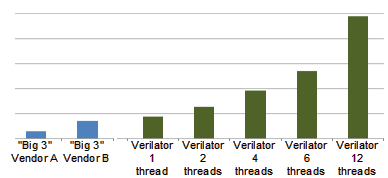
\includegraphics[scale=.7]{pictures/threads.png}
	\caption{Verilator creates highly threaded code \cite{veripool}}
	\end{center}
\end{figure}

\subsubsection{Co-Simulation Interface}
To effectively simulate the hard processor and the dedicated FPGA hardware logic\
ou co-simulation interface must support both an avalon bus master, slave, and an\
I2S master. The I2S master simulates the microphone data stream, which is a\
relatively simple sim routine. The hard processor is harder to simulate. Obviously\
we cannot fully simulate the hard cores because ARM HDL files\
are not made public. Further, the verilated design would be far too complicated to\
simulate with a reasonable speed. Thankfully we only use the HPS to read and write\
from the avalon bus and to do signal processing in C, which are all functions\
we can easily co-simulate without needing to run the actual ARM assembly.\
The avalon master can be simulated following the timing in figure \ref{avalon},\
and the I2S master can be simulated following the timing in figure \ref{i2s_timing}.\
Figure \ref{verilator} shows the high level block diagram for our current simulation\
setup. We believe that having an open source simulation setup is an important\
part of a complete open audio processing platform.

\begin{figure}[ht]
	\begin{center}
	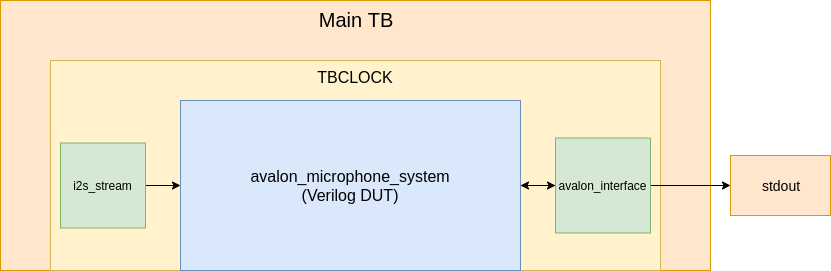
\includegraphics[scale=.3]{pictures/myblock.png}
	\caption{Verilator co-simulation architecture}
	\label{verilator}
	\end{center}
\end{figure}

\subsection{Continuous Recording}
One of our immediate goals is to expand the capabilities of our system to\
utilize more microphones. The current implementation will take samples from\
8 MEMS microphones and two channels from the line in port. This is a good\
starting point, but we want to be able to test algorithms on larger arrays.\
As mentioned in the ``DMA and Buffers'' section, the current implementation\
allocates 10 specific regions in DDR3 to store samples for a 90 second\
period. This works fine for 10 channels, and may even scale to more channels,\
but there is a finite amount of memory and eventually buffers will exceed\
the available memory. The solution to this problem is to use smaller\
buffers and offload them more often.

We have theorized a few ways to accomplish continuous recording, but we\
have decided using 100ms buffers per channel will be the most effective\
and the most flexible. We first considered sampling the microphones continuously\
without storing any information in buffers. This would work up to a large number\
of microphones because the FPGA fabric runs at a very fast speed relative to\
the frequency at which new samples are available (50 MHz vs. 48 KHz).\
In theory we could sample over 500 microphones in this manner.\
Unfortunately, some signal processing algorithms need to utilize the\
current sample along with previous samples. In order to do this we must\
keep some sort of buffer. We determined that 100ms is the longest time\
we would reasonably need to look back at.

\subsection{Replacing Altera\textsuperscript{\textregistered{}} Code}
Another goal we have is to replace as many Altera\textsuperscript{\textregistered{}}\
design blocks as we can. Generally speaking,\
Altera\textsuperscript{\textregistered{}}'s verilog is very difficult to\
work with. It is clear that their code is designed to only be touched by\
other Altera\textsuperscript{\textregistered{}} programs such as\
Platform Designer. The result of this design choice is code that is nearly\
unreadable by humans. We feel it is important to replace these sloppy\
pieces of code with our own if we want to have a truly open and robust\
platform.

\section{Conclusion}
We were able to make good progress this semester towards our short term\
goal of increasing the number of microphones we can support. Most of our effort on\
SoC development has been to this end. To accelerate our prototyping\
and make working outside of the lab easier, we developed a relatively competent\
simulation environment. This environment will make our algorithm\
development several times faster by allowing us to rapidly deploy\
new code and monitor every signal we may need. Beyond supporting more\
microphones, we will be creating more physical microphone array prototypes\
to evaluate the performance of different layouts. We also configured\
GNU/Linux development environments to net the best performance in\
Quartus\textsuperscript{\textregistered{}} and with our verilated\
designs. In conclusion, we had a very productive semester with significant\
progress towards speeding up development times, and we will be spending\
more time working on hardware features next semester.

\printbibliography

\end{document}